% Chapter Template

\chapter{Results and Discussion} % Main chapter title

\label{Chapter4} % Change X to a consecutive number; for referencing this chapter elsewhere, use \ref{ChapterX}

\lhead{Chapter 4. \emph{Results and Discussion}} % Change X to a consecutive number; this is for the header on each page - perhaps a shortened title

%----------------------------------------------------------------------------------------
%\t\tSECTION 1
%---------------------------------------------------------------------------------------
\section{Evaluation Metrics}

The performance of the vision-augmented AgentFormer was evaluated on the nuScenes dataset and compared against the baseline AgentFormer model. The standard metrics for motion forecasting, Average Displacement Error (ADE) and Final Displacement Error (FDE), were used for the evaluation.

\subsection{Average Displacement Error (ADE)}

Average Displacement Error (ADE) is a widely used metric for evaluating trajectory forecasting models. It measures the average L2 distance between the predicted trajectory and the ground truth trajectory over all predicted timesteps. For a predicted trajectory $\hat{Y} = (\hat{y}_1, \hat{y}_2, ..., \hat{y}_T)$ and a ground truth trajectory $Y = (y_1, y_2, ..., y_T)$, the ADE is calculated as:

\begin{equation}
ADE = \frac{1}{T} \sum_{t=1}^{T} ||\hat{y}_t - y_t||_2
\end{equation}

where $T$ is the prediction horizon and $||\cdot||_2$ denotes the L2 norm. A lower ADE value indicates a better forecasting performance.

\subsection{Final Displacement Error (FDE)}

Final Displacement Error (FDE) is another common metric for trajectory forecasting. It measures the L2 distance between the predicted final destination and the ground truth final destination at the end of the prediction horizon $T$. The FDE is calculated as:

\begin{equation}
FDE = ||\hat{y}_T - y_T||_2
\end{equation}

A lower FDE value indicates a better prediction of the agent's final position.

\section{Experiments}

This section details the experimental procedure for training and evaluating the baseline (vanilla) AgentFormer and the vision-augmented AgentFormer models.

\subsection{Vanilla AgentFormer}

The baseline AgentFormer model was trained and evaluated using the standard configuration provided in the original implementation. The model was trained on the nuScenes dataset using only the trajectory data. The following command was used to initiate the training process:

\begin{verbatim}
python train.py --cfg nuscenes\_5sample\_agentformer
\end{verbatim}

This command uses the \texttt{nuscenes\_5sample\_agentformer.yml} configuration file, which defines the model architecture, training parameters, and data paths for the vanilla AgentFormer.

\subsection{BEV-Augmented AgentFormer}

The vision-augmented AgentFormer model was trained using the pre-computed BEV features. The training process was initiated with the following command:

\begin{verbatim}
python train.py --cfg nuscenes\_5sample\_agentformer\_bev
\end{verbatim}

This command uses the \texttt{nuscenes\_5sample\_agentformer\_bev.yml} configuration file. This file is similar to the vanilla configuration but with the following key differences:

\begin{itemize}
    \item \texttt{use\_bev: true}: Enables the use of BEV features.
    \item \texttt{freeze\_bev\_encoder: true}: Freezes the BEV encoder weights.
    \item \texttt{use\_precomputed\_bev: true}: Instructs the data loader to load the pre-computed BEV features.
\end{itemize}

By using the pre-computed features, the training process is significantly accelerated as the model does not need to extract BEV features from the raw image data during training.

\section{Quantitative Results}

\begin{table}[h]
\centering
\caption{Performance comparison of baseline and vision-augmented AgentFormer.}
\label{tab:results}
\begin{tabular}{lcc}
\toprule
\textbf{Model} & \textbf{ADE} & \textbf{FDE} \\
\midrule
Baseline AgentFormer & 4.8110 & 9.5486 \\
Vision-Augmented AgentFormer & 5.1939 & 11.0132 \\
\bottomrule
\end{tabular}
\end{table}

As shown in Table \ref{tab:results}, the vision-augmented AgentFormer performed worse than the baseline model on both ADE and FDE metrics. This result is counter-intuitive, as the addition of visual information was expected to improve the model's performance. The following section provides a detailed analysis of the potential reasons for this performance degradation.

\subsection{Vanilla Model Training Loss}

Figure \ref{fig:loss_curves_vanilla} shows the training loss curves for the baseline AgentFormer model. The plots show the average loss per epoch for the total loss, KLD loss, reconstruction loss, and diversity loss.

\begin{figure}[h]
\centering
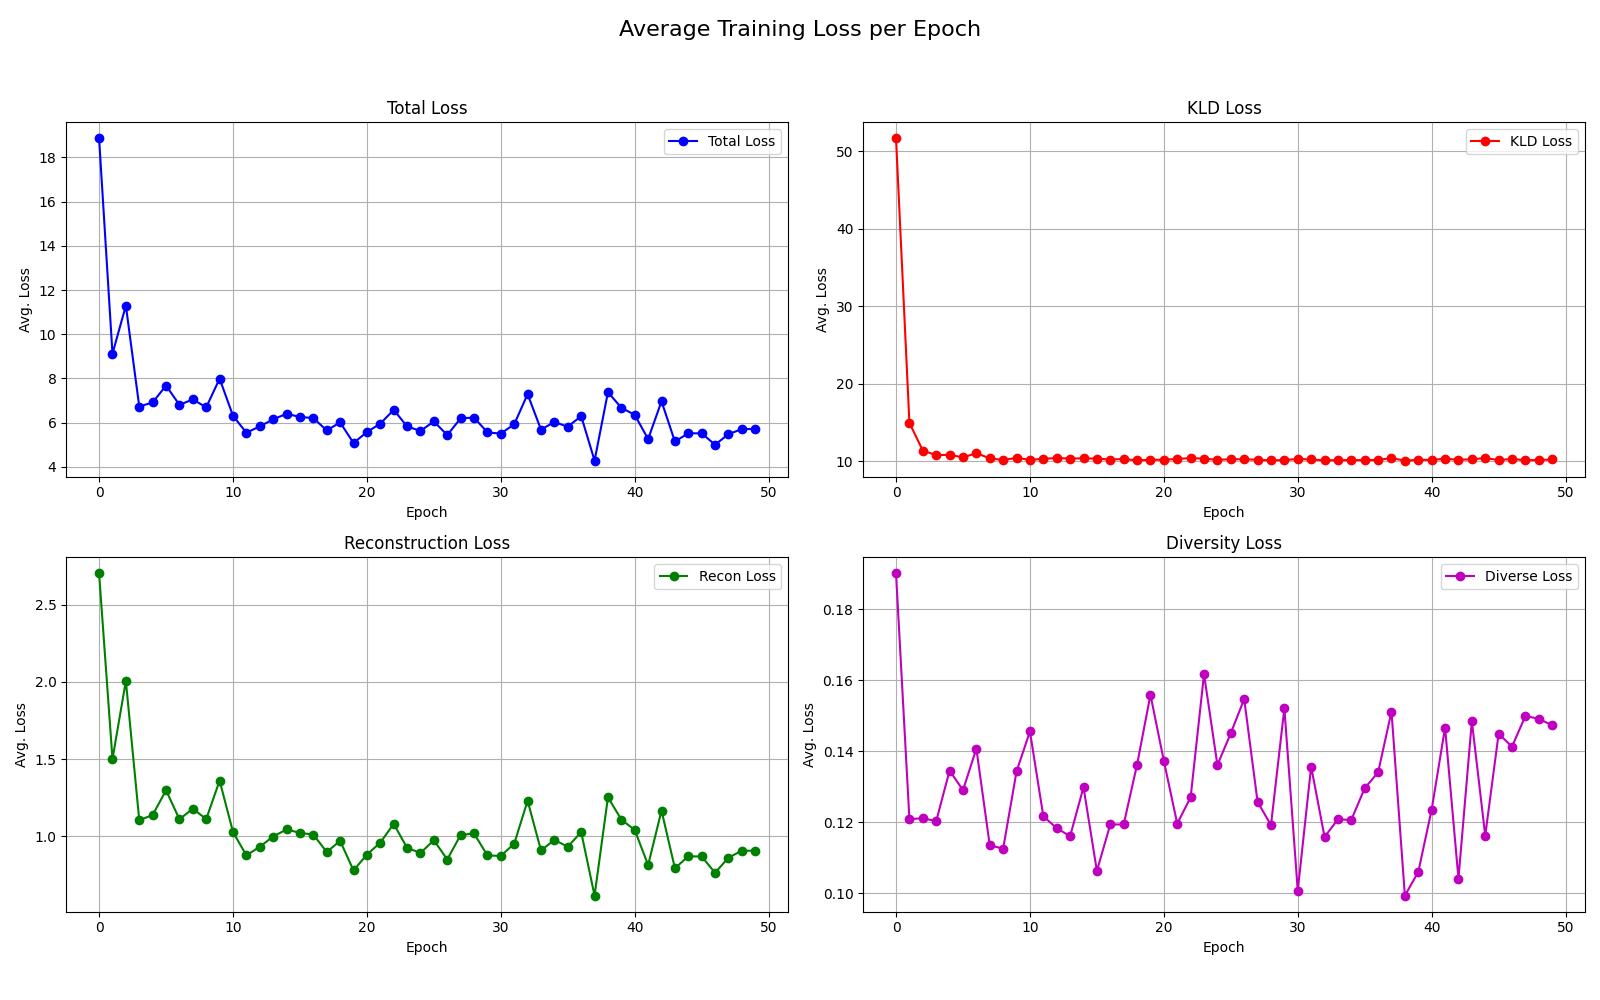
\includegraphics[width=\textwidth]{epoch_loss_curves_vanilla.png}
\caption{Average training loss per epoch for the baseline AgentFormer (Vanilla).}
\label{fig:loss_curves_vanilla}
\end{figure}

\subsection{BEV-Augmented Model Training Loss}

Figure \ref{fig:loss_curves_bev} shows the training loss curves for the vision-augmented AgentFormer model. The plots show the average loss per epoch for the total loss, KLD loss, MSE loss, and sample loss.

\begin{figure}[h]
\centering
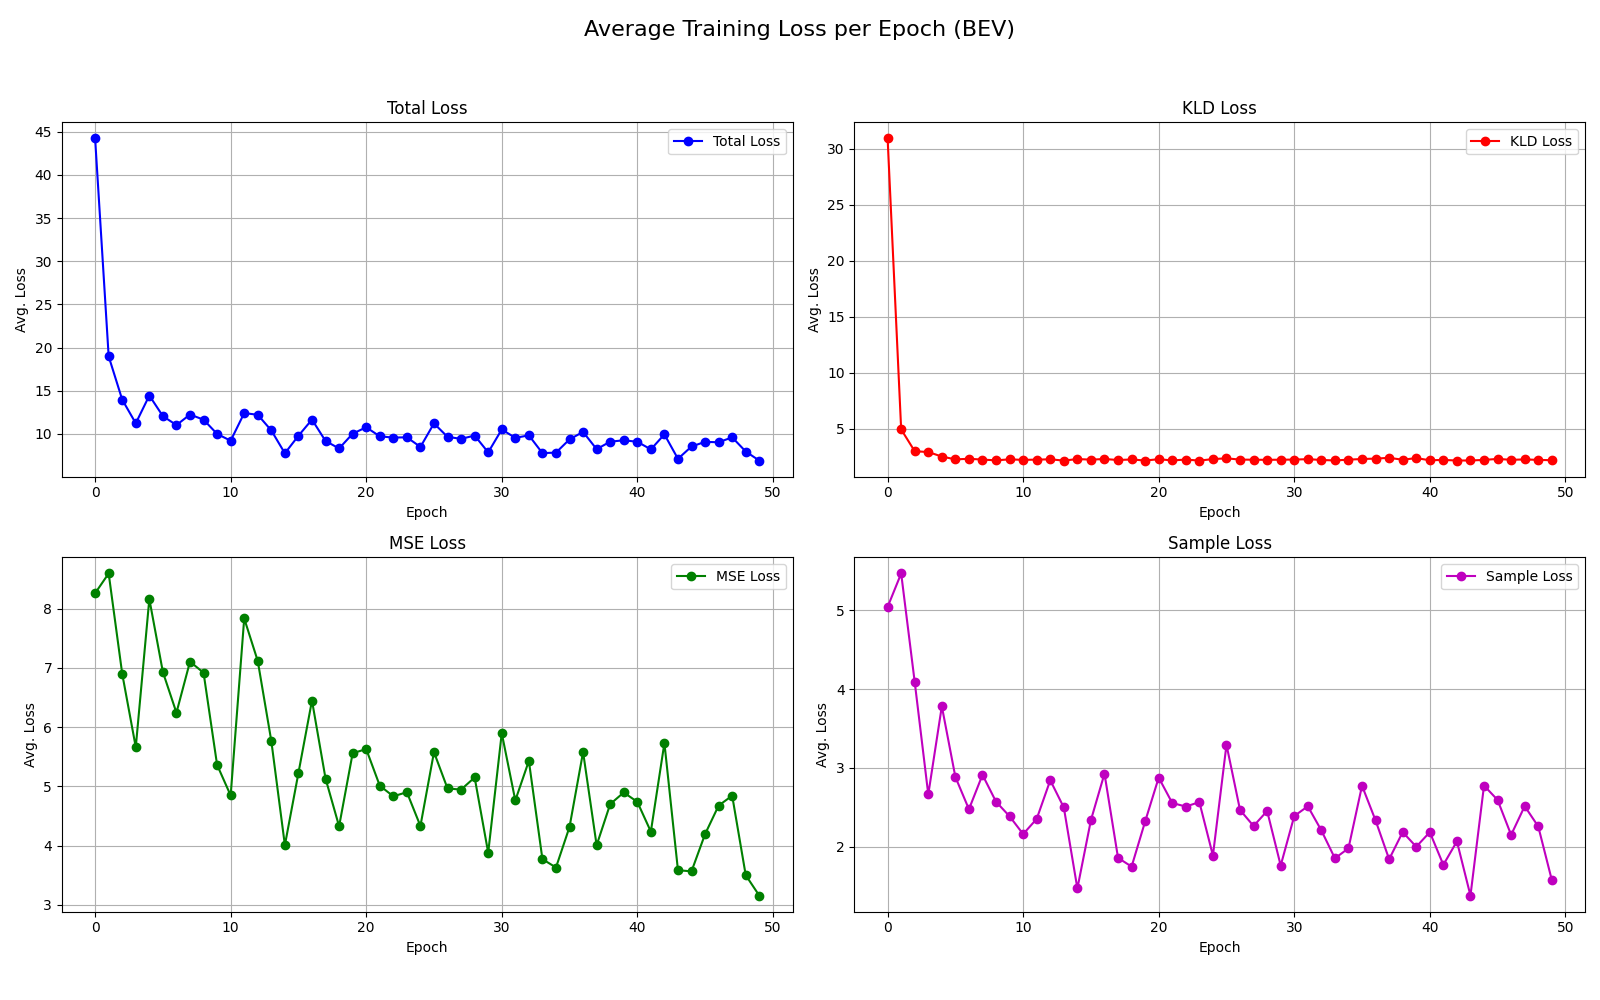
\includegraphics[width=\textwidth]{epoch_loss_curves_bev.png}
\caption{Average training loss per epoch for the vision-augmented AgentFormer (BEV).}
\label{fig:loss_curves_bev}
\end{figure}

\begin{itemize}
    \item \textbf{Total Loss:} The total loss is the sum of the other loss components. It shows a steep decrease in the first few epochs and then stabilizes, indicating that the model is learning. However, the final loss is still relatively high, which is consistent with the poor performance on the ADE and FDE metrics.
    \item \textbf{KLD Loss:} The Kullback-Leibler divergence (KLD) loss is part of the CVAE framework. It measures the difference between the learned latent distribution and the prior distribution. The KLD loss also shows a steep decrease in the beginning and then becomes stable. This indicates that the latent space is being learned correctly.
    \item \textbf{MSE Loss:} The Mean Squared Error (MSE) loss is the primary loss function for the trajectory prediction task. It measures the L2 distance between the predicted and ground truth trajectories. The MSE loss shows a decreasing trend, but with significant fluctuations. This volatility suggests that the model is struggling to find a stable solution. The high final value of the MSE loss is the main contributor to the high ADE and FDE scores.
    \item \textbf{Sample Loss:} The sample loss encourages the model to generate diverse samples. It also shows a decreasing trend with fluctuations, similar to the MSE loss.
\end{itemize}

The analysis of the loss curves provides further evidence for the suboptimal performance of the vision-augmented model. The instability in the MSE loss suggests that the model is not able to effectively integrate the visual information from the BEV features. The high variance in the loss indicates that for some training examples, the BEV features are helpful, while for others they are detrimental, leading to a high overall error. This is a strong indication that the fusion mechanism is not robust enough to handle the complexity of the multi-modal input.

\subsection{Comparative Analysis of Training Loss}

A comparison of the training loss curves for the vanilla and BEV-augmented models reveals a key difference in the training dynamics. While both models show a similar trend in the KLD and diversity/sample losses, the reconstruction/MSE loss behaves very differently.

The vanilla model's reconstruction loss shows a stable and consistent decrease, indicating that the model is effectively learning to reconstruct the ground truth trajectories. In contrast, the BEV-augmented model's MSE loss is highly volatile and fluctuates significantly throughout the training process. This suggests that the introduction of BEV features introduces a significant amount of noise and instability into the training process.

The higher and more unstable MSE loss of the BEV-augmented model is the primary reason for its worse performance compared to the vanilla model. The model is not able to effectively leverage the visual information from the BEV features and, in many cases, this information seems to be detrimental to the learning process. This further supports the hypothesis that a simple fusion mechanism is not sufficient to effectively combine the rich and dense BEV features with the sparse trajectory data.

\section{Analysis of Negative Results}

The unexpected negative results suggest that simply fusing BEV features with trajectory data is not sufficient to improve motion forecasting performance. This section explores several potential reasons for this outcome.

\subsection{Domain Mismatch}

The BEVDepth model was pre-trained on a large-scale dataset for 3D object detection. While this dataset is also from the autonomous driving domain, the distribution of scenes and the specific task it was trained on might be different from the motion forecasting task. This domain mismatch could lead to the BEV features not being optimally suited for trajectory prediction. The features that are important for object detection (e.g., precise object boundaries) might not be the most relevant for predicting future motion.

\subsection{Feature Incompatibility}

The BEV features are rich and dense, containing a vast amount of information about the scene. However, the AgentFormer model is primarily designed to work with sparse trajectory data. The simple fusion mechanism used in this project (concatenation followed by an MLP) might not be effective enough to bridge the gap between these two different modalities. The model might struggle to extract the relevant information from the dense BEV features and integrate it meaningfully with the trajectory information.

\subsection{Information Redundancy and Conflict}

The past trajectory of an agent already contains a significant amount of information about its future motion and the scene context (e.g., lane following behavior). The visual information from the BEV features might be redundant with this information. For example, if an agent is following a lane, its past trajectory already implies the lane geometry. The BEV features showing the same lane geometry might not add much new information. In the worst case, the visual information might even conflict with the trajectory information, leading to confusion and a decrease in performance.

\subsection{Sparsity of Relevant Information}

While the BEV map is dense, the information that is truly relevant for predicting the future motion of a specific agent might be very sparse. For example, the most important information might be the location of a traffic light, the presence of a pedestrian in a crosswalk, or the behavior of a single interacting vehicle. The model might struggle to identify these sparse but crucial pieces of information from the high-dimensional and noisy BEV feature map.

\subsection{Frozen BEV Encoder}

In this project, the BEV encoder was frozen to reduce the computational cost of training. This means that the BEV features were not fine-tuned for the motion forecasting task. The features that are optimal for object detection might not be optimal for trajectory prediction. Fine-tuning the BEV encoder on the motion forecasting task could allow it to learn features that are more relevant to the downstream task, potentially leading to better performance.

\subsection{Suboptimal Fusion Strategy}

The fusion strategy used in this project is a simple concatenation followed by an MLP. This is a common and straightforward approach, but it might not be the most effective way to fuse information from two different modalities. More sophisticated fusion techniques, such as cross-attention mechanisms, could be explored. Cross-attention would allow the model to selectively attend to the most relevant parts of the BEV feature map for each agent, potentially leading to a more effective fusion of information.
